\pagebreak
\chapter{Auktionshaus Auenland}

\begin{figure}[!ht]
    \centering
    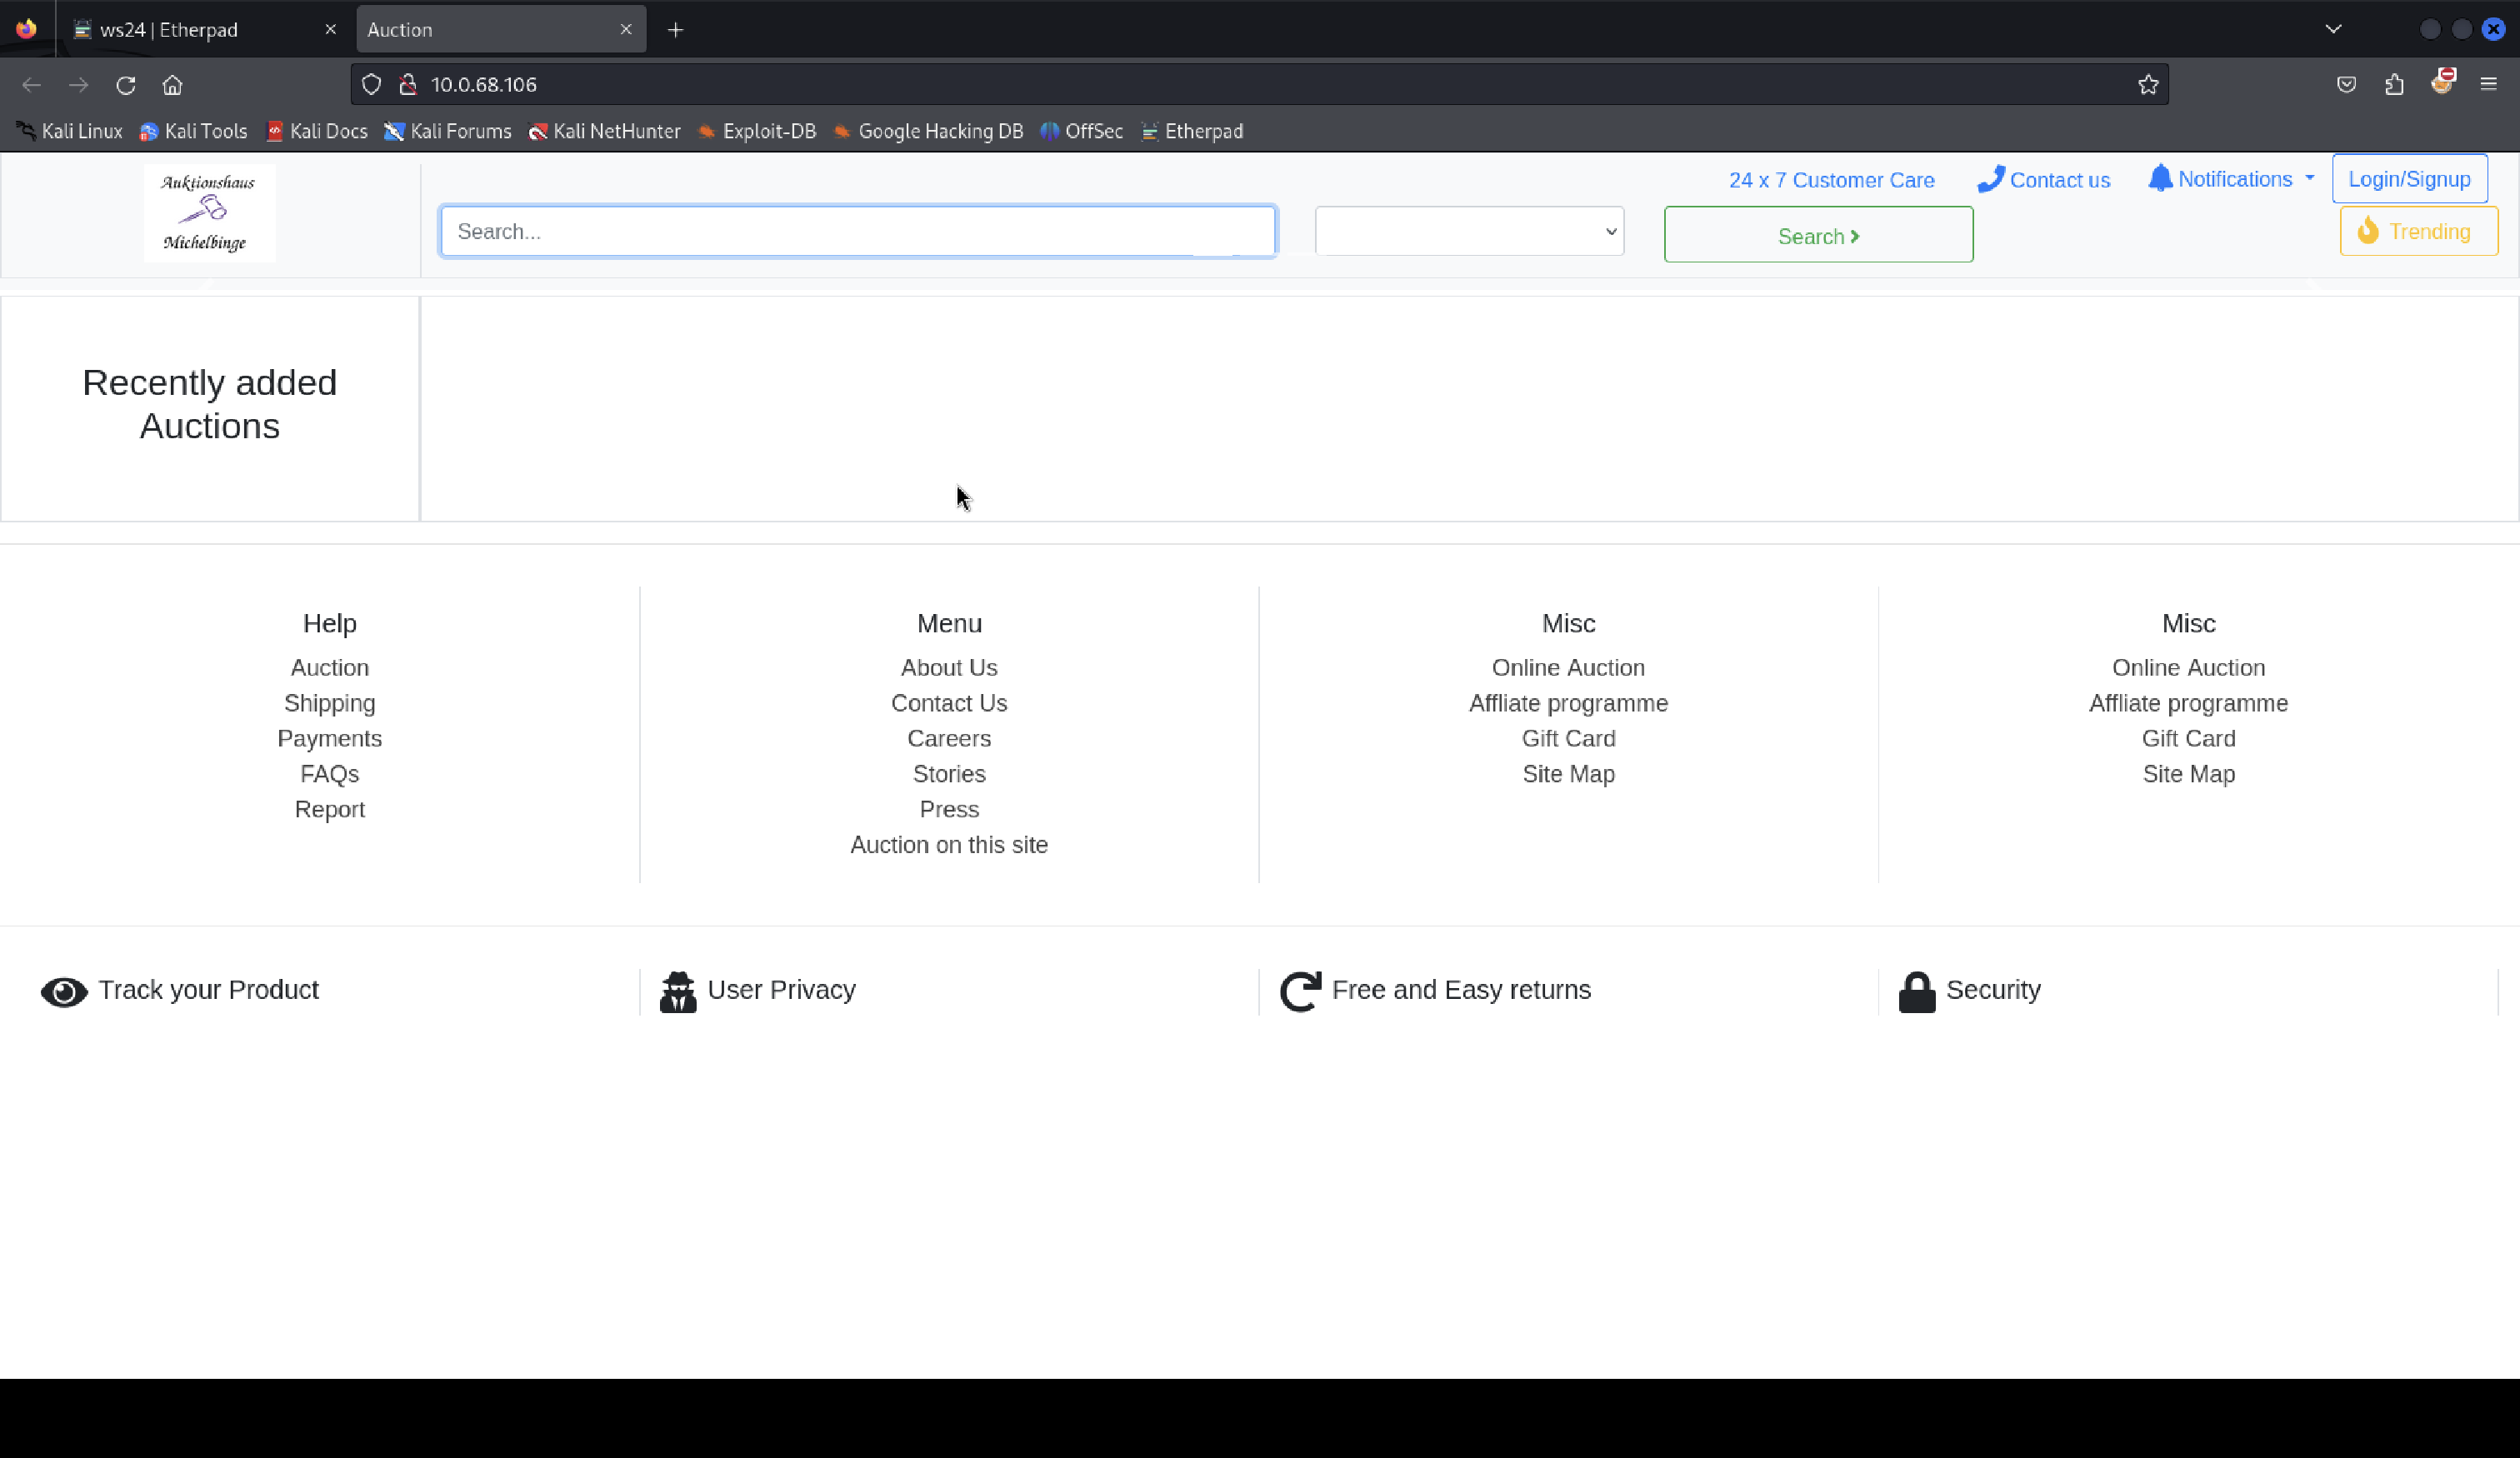
\includegraphics[width=\linewidth]{images/screenshots/08_auktionshaus.png}
    \caption{Webanwendung Auktionshaus Auenland}
    \label{fig:06_auktionshaus}
\end{figure}
\newpage

\cvss{av=network, ac=low, pr=none, ui=required, s=changed, c=high, i=high, a=high}
\cvssdescription{Etiam risus sapien, ornare at dui ut, semper eleifend arcu. In fermentum felis ut ornare convallis. Donec ultrices condimentum neque ut semper.}

\section{\makecvssbadge Auktionshaus Auenland: Upload einer Webshell}
\cvssaddtosummary{Auktionshaus Auenland: Upload einer Webshell}

\subsection*{Proof of concept}
Über das Login-Formular kann ein neuer Nutzer angelegt werden, dieser muss nicht durch einen Aministrator oder ähnlichem bestätigt werden, der Account ist sofort nach Erstellung aktiv. Mit dem erstellten Account kann ein Produkt zur Auktion freigegeben werden (unter der URL \url{http://10.0.68.106/sell_product.php}). Anstelle des Produktbildes kann eine PHP-Webshell hochgeladen werden. Die Auktion wird erstellt und in der Übersicht der aktiven Auktionen kann das Bild der zuvor erstellten Auktion in einem neuen Tab geöffnet werden. Dadurch öffnet sich die Webshell in einem neuen Tab und kann zur Ausführung von Kommandos verwendet werden.

\subsection*{Empfehlungen}

\cvss{av=network, ac=low, pr=none, ui=required, s=changed, c=high, i=high, a=high}
\cvssdescription{Etiam risus sapien, ornare at dui ut, semper eleifend arcu. In fermentum felis ut ornare convallis. Donec ultrices condimentum neque ut semper.}

\section{\makecvssbadge Auktionshaus Auenland: Reverse Shell}
\cvssaddtosummary{Auktionshaus Auenland: Reverse Shell}

\subsection*{Proof of concept}
\begin{figure}[!ht]
    \centering
    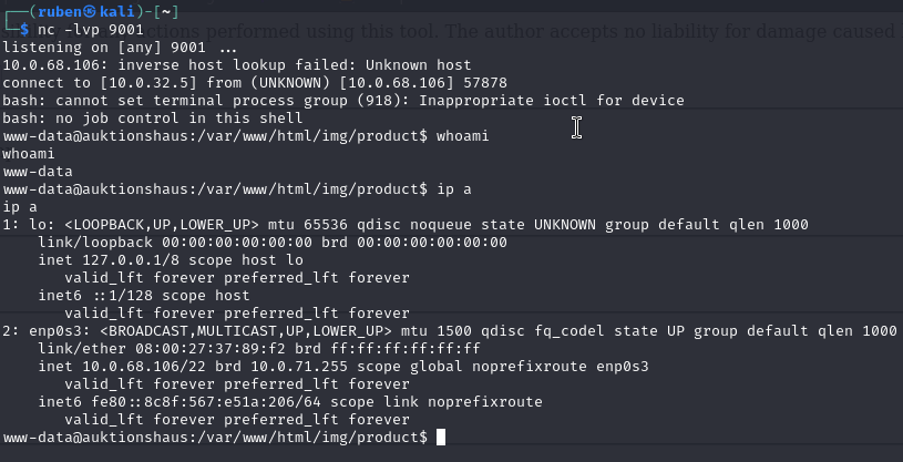
\includegraphics[width=\linewidth]{images/proofs/06_auktionshaus_proof.png}
    \caption{Proof für die Webanwendung Auktionshaus Auenland}
    \label{fig:06_auktionshaus_proof}
\end{figure}

\subsection*{Empfehlungen}